\chapter{GridWorld: Part 1}
\label{gridworld1}


\section{Getting started}

Now is a good time to start working with the AP Computer Science Case Study, which is a program called GridWorld.
To get started, install GridWorld, which you can download from the College Board:
\url{http://www.collegeboard.com/student/testing/ap/compsci_a/case.html}.

When you unpack this code, you should have a folder named {\tt GridWorldCode} that contains {\tt projects/firstProject}, which contains {\tt BugRunner.java}.

Make a copy of {\tt BugRunner.java} in another folder and then import it into your development environment.
There are instructions here that might help:
\url{http://www.collegeboard.com/prod_downloads/student/testing/ap/compsci_a/ap07_gridworld_installation_guide.pdf}.

Once you run {\tt BugRunner.java}, download the GridWorld Student Manual from:
\url{http://www.collegeboard.com/prod_downloads/student/testing/ap/compsci_a/ap07_gridworld_studmanual_appends_v3.pdf}.

The Student Manual uses vocabulary I have not presented yet, so to get you started, here is a quick preview:

\begin{itemize}

\item The components of GridWorld, including Bugs, Rocks and the Grid itself, are {\bf objects}.

\item A {\bf constructor} is a special method that creates new objects.

\item A {\bf class} is a set of objects; every object belongs to a class.

\item An object is also called an {\bf instance} because it is a member, or instance, of a class.

\item An {\bf attribute} is a piece of information about an object, like its color or location.

\item An {\bf accessor method} is a method that returns an attribute of an object.

\item A {\bf modifier method} changes an attribute of an object.

\end{itemize}

Now you should be able to read Part 1 of the Student Manual and do the exercises.


\section{BugRunner}

{\tt BugRunner.java} contains this code:

\begin{code}
import info.gridworld.actor.ActorWorld;
import info.gridworld.actor.Bug;
import info.gridworld.actor.Rock;

public class BugRunner
{
    public static void main(String[] args)
    {
        ActorWorld world = new ActorWorld();
        world.add(new Bug());
        world.add(new Rock());
        world.show();
    }
}
\end{code}

The first three lines are \java{import} statements; they list the classes from GridWorld used in this program.
You can find the documentation for these classes at \url{http://www.greenteapress.com/thinkapjava/javadoc/gridworld/}.

Like the other programs we have seen, BugRunner defines a class that provides a \java{main} method.
The first line of \java{main} creates an \java{ActorWorld} object.
\java{new} is a Java keyword that creates new objects.

The next two lines create a Bug and a Rock, and add them to \java{world}.
The last line shows the world on the screen.

Open {\tt BugRunner.java} for editing and replace this line:

\begin{code}
    world.add(new Bug());
\end{code}

with these lines:

\begin{code}
    Bug redBug = new Bug();
    world.add(redBug);
\end{code}

The first line assigns the Bug to a variable named \java{redBug}; we can use \java{redBug} to invoke the Bug's methods.
Try this:

\begin{code}
    System.out.println(redBug.getLocation());
\end{code}

Note: If you run this before adding the Bug to the \java{world}, the result is \java{null}, which means that the Bug doesn't have a location yet.

Invoke the other accessor methods and print the bug's attributes.
Invoke the methods \java{canMove}, \java{move} and \java{turn} and be sure you understand what they do.
% Now try these exercises:


\section{Exercises}


\begin{exercise}

\begin{enumerate}

\item Write a method named \java{moveBug} that takes a bug as a parameter and invokes \java{move}.
Test your method by calling it from \java{main}.

\item Modify \java{moveBug} so that it invokes \java{canMove} and moves the bug only if it can.

\item Modify \java{moveBug} so that it takes an integer, \java{n}, as a parameter, and moves the bug \java{n} times (if it can).

\item Modify \java{moveBug} so that if the bug can't move, it invokes \java{turn} instead.

\end{enumerate}
\end{exercise}


\begin{exercise}

\begin{enumerate}

\item The \java{Math} class provides a method named \java{random} that returns a double between 0.0 and 1.0 (not including 1.0).

\item Write a method named \java{randomBug} that takes a Bug as a parameter and sets the Bug's direction to one of 0, 90, 180 or 270 with equal probability, and then moves the bug if it can.

\item Modify \java{randomBug} to take an integer \java{n} and repeat \java{n} times.

The result is a random walk, which you can read about at \url{http://en.wikipedia.org/wiki/Random_walk}.

\item To see a longer random walk, you can give ActorWorld a bigger stage.
At the top of {\tt BugRunner.java}, add this \java{import} statement:

\begin{code}
import info.gridworld.grid.UnboundedGrid;
\end{code}

Now replace the line that creates the ActorWorld with this:

\begin{code}
    ActorWorld world = new ActorWorld(new UnboundedGrid());
\end{code}

You should be able to run your random walk for a few thousand steps (you might have to use the scrollbars to find the Bug).

\end{enumerate}
\end{exercise}


\begin{exercise}

GridWorld uses Color objects, which are defined in a Java library.
You can read the documentation at \url{http://download.oracle.com/javase/6/docs/api/java/awt/Color.html}.

To create Bugs with different colors, we have to import \java{Color}:

\begin{code}
import java.awt.Color;
\end{code}

Then you can access the predefined colors, like \java{Color.blue}, or create a new color like this:

\begin{code}
    Color purple = new Color(148, 0, 211);
\end{code}

Make a few bugs with different colors.
Then write a method named \java{colorBug} that takes a Bug as a parameter, reads its location, and sets the color.

The Location object you get from \java{getLocation} has methods named \java{getRow} and \java{getCol} that return integers.
So you can get the x-coordinate of a Bug like this:

\begin{code}
    int x = bug.getLocation().getCol();
\end{code}

Write a method named \java{makeBugs} that takes an ActorWorld and an integer \java{n} and creates \java{n} bugs colored according to their location.
Use the row number to control the red level and the column to control the blue.

\end{exercise}


\chapter{GridWorld: Part 2}
\label{gridworld2}


\section{BoxBug}

Part 2 of the GridWorld case study uses some features we haven't seen yet, so you will get a preview now and more details later.
As a reminder, you can find the documentation for the GridWorld classes at \url{http://www.greenteapress.com/thinkapjava/javadoc/gridworld/}.

When you install GridWorld, you should have a folder named {\tt projects/boxBug}, which contains {\tt BoxBug.java}, {\tt BoxBugRunner.java} and {\tt BoxBug.gif}.

Copy these files into your working folder and import them into your development environment.
There are instructions here that might help:
\url{http://www.collegeboard.com/prod_downloads/student/testing/ap/compsci_a/ap07_gridworld_installation_guide.pdf}.

Here is the code from {\tt BoxBugRunner.java}:

\begin{code}
import info.gridworld.actor.ActorWorld;
import info.gridworld.grid.Location;

import java.awt.Color;

public class BoxBugRunner {
    public static void main(String[] args) {
        ActorWorld world = new ActorWorld();
        BoxBug alice = new BoxBug(6);
        alice.setColor(Color.ORANGE);
        BoxBug bob = new BoxBug(3);
        world.add(new Location(7, 8), alice);
        world.add(new Location(5, 5), bob);
        world.show();
    }
}
\end{code}

Everything here should be familiar, with the possible exception of \java{Location}, which is part of GridWorld, and similar to \java{java.awt.Point}.

{\tt BoxBug.java} contains the class definition for BoxBug.

\begin{code}
public class BoxBug extends Bug {
    private int steps;
    private int sideLength;

    public BoxBug(int length) {
        steps = 0;
        sideLength = length;
    }
}
\end{code}

The first line says that this class extends \java{Bug}, which means that a \java{BoxBug} is a kind of \java{Bug}.

The next two lines are instance variables.
Every \java{Bug} has variables named \java{sideLength}, which determines the size of the box it draws, and \java{steps}, which keeps track of how many steps the \java{Bug} has taken.

The next line defines a {\bf constructor}, which is a special method that initializes the instance variables.
When you create \java{Bug} by invoking \java{new}, Java invokes this constructor.

The parameter of the constructor is the side length.

\java{Bug} behavior is controlled by the \java{act} method.
Here is the \java{act} method for \java{BoxBug}:

\begin{code}
    public void act() {
        if (steps < sideLength && canMove()) {
            move();
            steps++;
        }
        else {
            turn();
            turn();
            steps = 0;
        }
    }
\end{code}

If the \java{BoxBug} can move, and has not taken the required number of steps, it moves and increments \java{steps}.

If it hits a wall or completes one side of the box, it turns 90 degrees to the right and resets \java{steps} to 0.

Run the program and see what it does.
Did you get the behavior you expected?


\section{Termites}

I wrote a class called \java{Termite} that extends \java{Bug} and adds the ability to interact with flowers.
To run it, download these files and import them into your development environment:

\url{http://thinkapjava.com/code/Termite.java} \\
\url{http://thinkapjava.com/code/Termite.gif} \\
\url{http://thinkapjava.com/code/TermiteRunner.java} \\
\url{http://thinkapjava.com/code/EternalFlower.java}

Because \java{Termite} extends \java{Bug}, all \java{Bug} methods also work on \java{Termite}s.
But \java{Termite}s have additional methods that \java{Bug}s don't have.

\begin{code}
    /**
     * Returns true if the termite has a flower.
     */
    public boolean hasFlower();

    /**
     * Returns true if the termite is facing a flower.
     */
    public boolean seeFlower();

    /**
     * Creates a flower unless the termite already has one.
     */
    public void createFlower();

    /**
     * Drops the flower in the termites current location.
     *
     * Note: only one Actor can occupy a grid cell, so the effect
     * of dropping a flower is delayed until the termite moves.
     */
    public void dropFlower();

    /**
     * Throws the flower into the location the termite is facing.
     */
    public void throwFlower();

    /**
     * Picks up the flower the termite is facing, if there is
     * one, and if the termite doesn't already have a flower.
     */
    public void pickUpFlower();
\end{code}

For some methods \java{Bug} provides one definition and \java{Termite} provides another.
In that case, the \java{Termite} method {\bf overrides} the \java{Bug} method.

For example, \java{Bug.canMove} returns \java{true} if there is a flower in the next location, so \java{Bug}s can trample \java{Flower}s.
\java{Termite.canMove} returns \java{false} if there is any object in the next location, so \java{Termite} behavior is different.

As another example, Termites have a version of \java{turn} that takes an integer number of degrees as a parameter.
Finally, Termites have \java{randomTurn}, which turns left or right 45 degrees at random.

Here is the code from {\tt TermiteRunner.java}:

\begin{code}
public class TermiteRunner
{
    public static void main(String[] args)
    {
        ActorWorld world = new ActorWorld();
        makeFlowers(world, 20);

        Termite alice = new Termite();
        world.add(alice);

        Termite bob = new Termite();
        bob.setColor(Color.blue);
        world.add(bob);

        world.show();
    }

    public static void makeFlowers(ActorWorld world, int n) {
        for (int i = 0; i<n; i++) {
            world.add(new EternalFlower());
        }
    }
}
\end{code}

Everything here should be familiar.
\java{TermiteRunner} creates an \java{ActorWorld} with 20 \java{EternalFlowers} and two \java{Termites}.

An \java{EternalFlower} is a \java{Flower} that overrides \java{act} so the flowers don't get darker.

\begin{code}
public class EternalFlower extends Flower {
    public void act() {}
}
\end{code}

If you run {\tt TermiteRunner.java} you should see two termites moving at random among the flowers.

{\tt MyTermite.java} demonstrates the methods that interact with flowers.
Here is the class definition:

\begin{code}
public class MyTermite extends Termite {

    public void act() {
        if (getGrid() == null)
            return;

        if (seeFlower()) {
            pickUpFlower();
        }
        if (hasFlower()) {
            dropFlower();
        }

        if (canMove()) {
            move();
        }
        randomTurn();
    }
}
\end{code}

\java{MyTermite} extends \java{Termite} and overrides \java{act}.
If \java{MyTermite} sees a flower, it picks it up.
If it has a flower, it drops it.


\section{Langton's Termite}

Langton's Ant is a simple model of ant behavior that displays surprisingly complex behavior.
The Ant lives on a grid like GridWorld where each cell is either white or black.
The Ant moves according to these rules:

\begin{itemize}

\item If the Ant is on a white cell, it turns to the right, makes the cell black, and moves forward.

\item If the Ant is on a black cell, it turns to the left, makes the cell white, and moves forward.

\end{itemize}

Because the rules are simple, you might expect the Ant to do something simple like make a square or repeat a simple pattern.
But starting on a grid with all white cells, the Ant makes more than 10,000 steps in a seemingly random pattern before it settles into a repeating loop of 104 steps.

You can read more about Langton's Ant at \url{http://en.wikipedia.org/wiki/Langton_ant}.

It is not easy to implement Langton's Ant in GridWorld because we can't set the color of the cells.
As an alternative, we can use Flowers to mark cells, but we can't have an Ant and a Flower in the same cell, so we can't implement the Ant rules exactly.

Instead we'll create what I'll call a \java{LangtonTermite}, which uses \java{seeFlower} to check whether there is a flower in the next cell, \java{pickUpFlower} to pick it up, and \java{throwFlower} to put a flower in the next cell.
You might want to read the code for these methods to be sure you know what they do.


\section{Exercises}


\begin{exercise}
Now you know enough to do the exercises in the Student Manual, Part 2.
Go do them, and then come back for more fun.
\end{exercise}


\begin{exercise}
The purpose of this exercise is to explore the behavior of Termites that interact with flowers.

Modify {\tt TermiteRunner.java} to create \java{MyTermites} instead of \java{Termites}.
Then run it again.
\java{MyTermites} should move around at random, moving the flowers around.
The total number of flowers should stay the same (including the ones \java{MyTermites} are holding).

In {\em Termites, Turtles and Traffic Jams}, Mitchell Resnick describes a simple model of termite behavior:

\begin{itemize}

\item If you see a flower, pick it up.
Unless you already have a flower; in that case, drop the one you have.

\item Move forward, if you can.

\item Turn left or right at random.

\end{itemize}

Modify {\tt MyTermite.java} to implement this model.
What effect do you think this change will have on the behavior of \java{MyTermites}?

Try it out.
Again, the total number of flowers does not change, but over time the flowers accumulate in a small number of piles, often just one.

This behavior is an {\bf an emergent property}, which you can read about at \url{http://en.wikipedia.org/wiki/Emergence}.
\java{MyTermites} follow simple rules using only small-scale information, but the result is large-scale organization.

Experiment with different rules and see what effect they have on the system.
Small changes can have unpredicable results!

\end{exercise}


\begin{exercise}

\begin{enumerate}

\item Make a copy of {\tt Termite.java} called \java{LangtonTermite} and a copy of {\tt TermiteRunner.java} called {\tt LangtonRunner.java}.
Modify them so the class definitions have the same name as the files, and so \java{LangtonRunner} creates a \java{LangtonTermite}.

\item If you create a file named {\tt LangtonTermite.gif}, GridWorld uses it to represent your Termite.
You can download excellent pictures of insects from \url{http://www.cksinfo.com/animals/insects/realisticdrawings/index.html}.
To convert them to GIF format, you can use an application like ImageMagick.

\item Modify \java{act} to implement rules similar to Langton's Ant.
Experiment with different rules, and with both 45 and 90 degree turns.
Find rules that run the maximum number of steps before the Termite starts to loop.

\item To give your Termite enough room, you can make the grid bigger or switch to an \java{UnboundedGrid}.

\item Create more than one \java{LangtonTermite} and see how they interact.

\end{enumerate}

\end{exercise}


\chapter{GridWorld: Part 3}
\label{gridworld3}

If you haven't done the exercises in Chapters~\ref{gridworld1} and \ref{gridworld2}, you should do them before reading this chapter.
As a reminder, you can find the documentation for the GridWorld classes at \url{http://www.greenteapress.com/thinkapjava/javadoc/gridworld/}.

Part 3 of the GridWorld Student Manual presents the classes that make up GridWorld and the interactions among them.
It is an example of object-oriented design and an opportunity to discuss OO design issues.

But before you read the Student Manual, there are a few more things you need to know.


\section{ArrayList}

GridWorld uses \java{java.util.ArrayList}, which is an object similar to an array.
It is a {\bf collection}, which means that it's an object that contains other objects.
Java provides other collections with different capabilities, but to use GridWorld we only need \java{ArrayList}s.

To see an example, download \url{http://thinkapjava.com/code/BlueBug.java} and \url{http://thinkapjava.com/code/BlueBugRunner.java}.
A \java{BlueBug} is a bug that moves at random and looks for rocks.
If it finds a rock, it makes it blue.

Here's how it works.
When \java{act} is invoked, \java{BlueBug} gets its location and a reference to the grid:

\begin{code}
    Location loc = getLocation();
    Grid<Actor> grid = getGrid();
\end{code}

The type in angle-brackets (\verb"<>") is a {\bf type parameter} that specifies the contents of \java{grid}.
In other words, \java{grid} is not just a \java{Grid}, it's a \java{Grid} that contains \java{Actor}s.

The next step is to get the neighbors of the current location.
\java{Grid} provides a method that does just that:

\begin{code}
    ArrayList<Actor> neighbors = grid.getNeighbors(loc);
\end{code}

The return value from \java{getNeighbors} is an \java{ArrayList} of \java{Actors}.
The \java{size} method returns the length of the \java{ArrayList}, and \java{get} selects an element.
So we can print the neighbors like this.

\begin{code}
        for (int i = 0; i < neighbors.size(); i++) {
            Actor actor = neighbors.get(i);
            System.out.println(actor);
        }
\end{code}

Traversing an \java{ArrayList} is such a common operation there's a special syntax for it: the {\bf for-each loop}.
So we could write:

\begin{code}
        for (Actor actor : neighbors) {
            System.out.println(actor);
        }
\end{code}

We know that the neighbors are \java{Actors}, but we don't know what kind: they could be \java{Bug}s, \java{Rock}s, etc.
To find the Rocks, we use the \java{instanceof} operator, which checks whether an object is an instance of a class.

\begin{code}
        for (Actor actor : neighbors) {
            if (actor instanceof Rock) {
                actor.setColor(Color.blue);
            }
        }
\end{code}

To make all this work, we need to import the classes we use:

\begin{code}
import info.gridworld.actor.Actor;
import info.gridworld.actor.Bug;
import info.gridworld.actor.Rock;
import info.gridworld.grid.Grid;
import info.gridworld.grid.Location;

import java.awt.Color;
import java.util.ArrayList;
\end{code}


\section{Interfaces}
\index{interface}

GridWorld also uses Java {\bf interfaces}, so I want to explain what they are.
``Interface'' means different things in different contexts, but in Java it refers to a specific language feature: an interface is a class definition where the methods have no bodies.

In a normal class definition, each method has a prototype and a body (see Section~\ref{documentation}).
A prototype is also called a {\bf specification} because it specifies the name, parameters, and return type of the method.
The body is called the {\bf implementation} because it implements the specification.

In a Java interface the methods have no bodies, so it specifies the methods without implementing them.

For example, \java{java.awt.Shape} is an interface with prototypes for \java{contains}, \java{intersects}, and several other methods.
\java{java.awt.Rectangle} provides implementations for those methods, so we say that ``Rectangle implements Shape.''
In fact, the first line of the \java{Rectangle} class definition is:

\begin{code}
public class Rectangle extends Rectangle2D implements Shape, Serializable
\end{code}

Rectangle inherits methods from \java{Rectangle2D} and provides implementations for the methods in \java{Shape} and \java{Serializable}.

In GridWorld the Location class implements the \java{java.lang.Comparable} interface by providing \java{compareTo}, which is similar to \java{compareCards} in Section~\ref{compare}.
%
GridWorld also defines a new interface, \java{Grid}, that specifies the methods a \java{Grid} should provide.
And it includes two implementations, \java{BoundedGrid} and \java{UnboundedGrid}.

The Student Manual uses the abbreviation {\bf API}, which stands for ``application programming interface.''
The API is the set of methods that are available for you, the application programmer, to use.
See \url{http://en.wikipedia.org/wiki/Application_programming_interface}.


\section{Public and private}

Remember in Chapter~\ref{chap01} I said I would explain why the \java{main} method has the keyword \java{public}?
Finally, the time has come.

\java{public} means that the method can be invoked from other classes.
The alternative is \java{private}, which means the method can only be invoked inside the class where it is defined.

Instance variables can also be \java{public} or \java{private}, with the same result: a private instance variable can be accessed only inside the class where it is defined.

The primary reason to make methods and instance variables private is to limit interactions between classes in order to manage complexity.

For example, the Location class keeps its instance variables private.
It has accessor methods \java{getRow} and \java{getCol}, but it provides no methods that modify the instance variables.
In effect, Location objects are immutable, which means that they can be shared without worrying about unexpected behavior due to aliasing.

Making methods private helps keep the API simple.
Classes often include helper methods that are used to implement other methods, but making those methods part of the public API might be unnecessary and error-prone.

Private methods and instance variables are language features that help programmers ensure {\bf data encapsulation}, which means that objects in one class are isolated from other classes.


\section{Game of Life}

The mathematician John Conway invented the ``Game of Life,'' which he called a ``zero-player game'' because no players are needed to choose strategies or make decisions.
After you set up the initial conditions, you watch the game play itself.
But that turns out to be more interesting than it sounds; you can read about it at \url{http://en.wikipedia.org/wiki/Conways_Game_of_Life}.

The goal of this exercise is to implement the Game of Life in GridWorld.
The game board is the grid, and the pieces are Rocks.

The game proceeds in turns, or {\bf time steps}.
At the beginning of the time step, each Rock is either ``alive'' or ``dead''.
On the screen, the color of the Rock indicates its status.
%
The status of each Rock depends on the status of its {\bf neighbors}.
Each Rock has 8 neighbors, except the Rocks along the edge of the Grid.
Here are the rules:

\begin{itemize}

\item If a dead Rock has exactly three neighbors, it comes to life!
Otherwise it stays dead.

\item If a live Rock has 2 or 3 neighbors, it survives.
Otherwise it dies.

\end{itemize}

There are several consequences of these rules.
If all Rocks are dead, no Rocks come to life.
If you start with a single live Rock, it dies.
But if you have 4 Rocks in a square, they keep each other alive, so that's a stable configuration.

Most simple starting configurations either die out quickly or reach a stable configuration.
But there are a few starting conditions that display remarkable complexity.
One of those is the r-pentomino: it starts with only 5 Rocks, runs for 1103 timesteps and ends in a stable configuration with 116 live Rocks (see \url{http://www.conwaylife.com/wiki/R-pentomino}).

The following sections are suggestions for implementing Game of Life in GridWorld.
You can download my solution at \url{http://thinkapjava.com/code/LifeRunner.java} and \url{http://thinkapjava.com/code/LifeRock.java}.


\section{LifeRunner}

Make a copy of \java{BugRunner.java} named \java{LifeRunner.java} and add methods with the following prototypes:

\begin{code}
    /**
     * Makes a Game of Life grid with an r-pentomino.
     */
    public static void makeLifeWorld(int rows, int cols)

    /**
     * Fills the grid with LifeRocks.
     */
    public static void makeRocks(ActorWorld world)
\end{code}

\java{makeLifeWorld} should create a Grid of Actors and an ActorWorld, then invoke \java{makeRocks}, which should put a \java{LifeRock} at every location in the Grid.


\section{LifeRock}

Make a copy of \java{BoxBug.java} named \java{LifeRock.java}.
\java{LifeRock} should extend \java{Rock}.
Add an \java{act} method that does nothing.
At this point you should be able to run the code and see a Grid full of Rocks.

To keep track of the status of the Rocks, you can add a new instance variable, or you can use the Color of the Rock to indicate status.
Either way, write methods with these prototypes:

\begin{code}
    /**
     * Returns true if the Rock is alive.
     */
    public boolean isAlive()

    /**
     * Makes the Rock alive.
     */
    public void setAlive()

    /**
     * Makes the Rock dead.
     */
    public void setDead()
\end{code}

Write a constructor that invokes \java{setDead} and confirm that all Rocks are dead.


\section{Simultaneous updates}

In the Game of Life, all Rocks are updated simultaneously; that is, each rock checks the status of its neighbors before any Rocks change their status.
Otherwise the behavior of the system would depend on the order of the updates.

In order to implement simultaneous updates, I suggest that you write an \java{act} method that has two phases: during the first phase, all Rocks count their neighbors and record the results; during the second phase, all Rocks update their status.

Here's what my \java{act} method looks like:

\begin{code}
    /**
     * Check what phase we're in and calls the appropriate method.
     * Moves to the next phase.
     */
    public void act() {
        if (phase == 1) {
            numNeighbors = countLiveNeighbors();
            phase = 2;
        } else {
            updateStatus();
            phase = 1;
        }
    }
\end{code}

\java{phase} and \java{numNeighbors} are instance variables.
And here are the prototypes for \java{countLiveNeighbors} and \java{updateStatus}:

\begin{code}
    /**
     * Counts the number of live neighbors.
     */
    public int countLiveNeighbors()

    /**
     * Updates the status of the Rock (live or dead) based on
     * the number of neighbors.
     */
    public void updateStatus()
\end{code}

Start with a simple version of \java{updateStatus} that changes live rocks to dead and vice versa.
Now run the program and confirm that the Rocks change color.
Every two steps in the World correspond to one timestep in the Game of Life.

Now fill in the bodies of \java{countLiveNeighbors} and \java{updateStatus} according to the rules and see if the system behaves as expected.


\section{Initial conditions}

To change the initial conditions, you can use the GridWorld pop-up menus to set the status of the Rocks by invoking \java{setAlive}.
Or you can write methods to automate the process.

In \java{LifeRunner}, add a method called \java{makeRow} that creates an initial configuration with \java{n} live Rocks in a row in the middle of the grid.
What happens for different values of \java{n}?

Add a method called \java{makePentomino} that creates an r-pentomino in the middle of the Grid.
The initial configuration should look like this:

\begin{center}
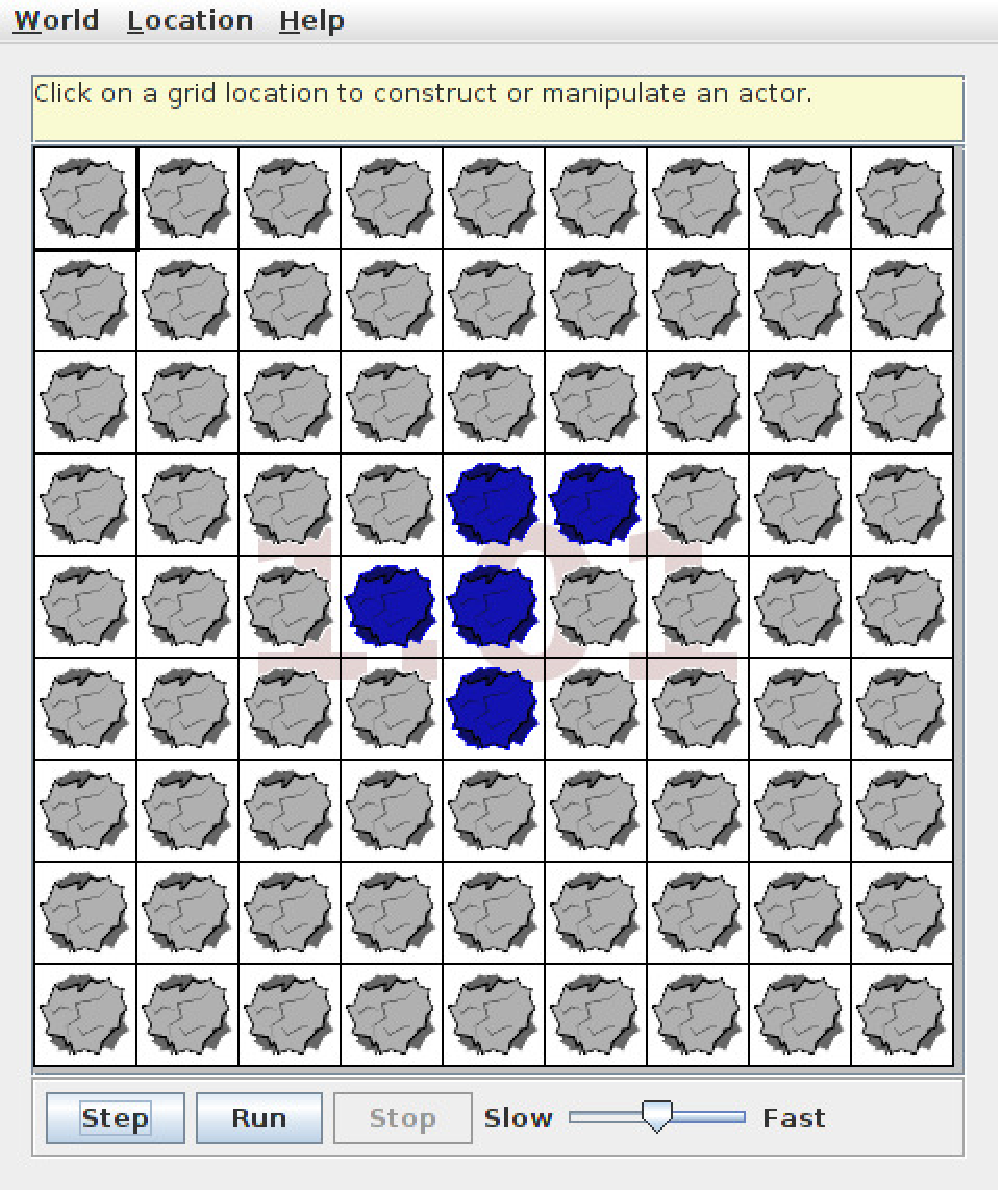
\includegraphics[height=2in]{figs/LifeRunner.pdf}
\end{center}

If you run this configuration for more than a few steps, it reaches the end of the Grid.
The boundaries of the Grid change the behavior of the system; in order to see the full evolution of the r-pentomino, the Grid has to be big enough.
You might have to experiment to find the right size, and depending on the speed of your computer, it might take a while.

The Game of Life web page describes other initial conditions that yield interesting results (\url{http://www.conwaylife.com/}).
Choose one you like and implement it.

There are also variations of the Game of Life based on different rules.
Try one out and see if you find anything interesting.


\section{Exercises}


\begin{exercise}
Starting with a copy of {\tt BlueBug.java}, write a class definition for a new kind of \java{Bug} that finds and eats flowers.
You can ``eat'' a flower by invoking \java{removeSelfFromGrid} on it.
\end{exercise}


\begin{exercise}
Now you know what you need to know to read Part 3 of the GridWorld Student Manual and do the exercises.
\end{exercise}


\begin{exercise}
If you implemented the Game of Life, you are well prepared for Part 4 of the GridWorld Student Manual.
Read it and do the exercises.
\end{exercise}


Congratulations, you're done!
